\documentclass[border=14pt]{standalone}
\usepackage[T1]{fontenc}
\usepackage[scaled]{helvet}
\renewcommand\familydefault\sfdefault
\usepackage{tikz}
\usetikzlibrary{arrows.meta,calc,positioning}
\definecolor{personF}{HTML}{F8E0A8}\definecolor{personD}{HTML}{B8860B}
\definecolor{slackF}{HTML}{DCE8F6}\definecolor{slackD}{HTML}{5B7FA8}
\definecolor{sessF}{HTML}{CDE8E1}\definecolor{sessD}{HTML}{2E8B74}
\definecolor{subF}{HTML}{E6DDF3}\definecolor{subD}{HTML}{7E5DB8}
\definecolor{workF}{HTML}{E1EECD}\definecolor{workD}{HTML}{6A9A3A}
\definecolor{servF}{HTML}{E6E8EB}\definecolor{servD}{HTML}{8A9099}
\definecolor{codeF}{HTML}{F6DAD6}\definecolor{codeD}{HTML}{C0605A}
\definecolor{arrC}{HTML}{6B7280}\definecolor{labC}{HTML}{555B66}
\tikzset{
  box/.style={rounded corners=3pt, draw, line width=0.8pt, align=center, text width=3.4cm,
              inner sep=5pt, minimum height=1.2cm, font=\normalsize},
  person/.style={box, fill=personF, draw=personD},
  slack/.style={box, fill=slackF, draw=slackD},
  sess/.style={box, fill=sessF, draw=sessD},
  sub/.style={box, fill=subF, draw=subD},
  work/.style={box, fill=workF, draw=workD},
  serv/.style={box, fill=servF, draw=servD},
  code/.style={box, fill=codeF, draw=codeD},
  arr/.style={-{Stealth[length=2.4mm,width=1.8mm]}, draw=arrC, line width=0.8pt},
  lab/.style={font=\small\itshape, text=labC, fill=white, inner sep=1.5pt},
}
\hyphenpenalty=10000 \exhyphenpenalty=10000
\newcommand\nd[2]{\textbf{#1}\\[1pt]{\small #2}}
\newcommand\titled[2]{\node[anchor=south west, inner sep=0pt] at ($(current bounding box.north west)+(0cm,0.45cm)$)
  {{\bfseries\LARGE #1}\hspace{1.2em}{\color{labC}\large #2}};}
\begin{document}
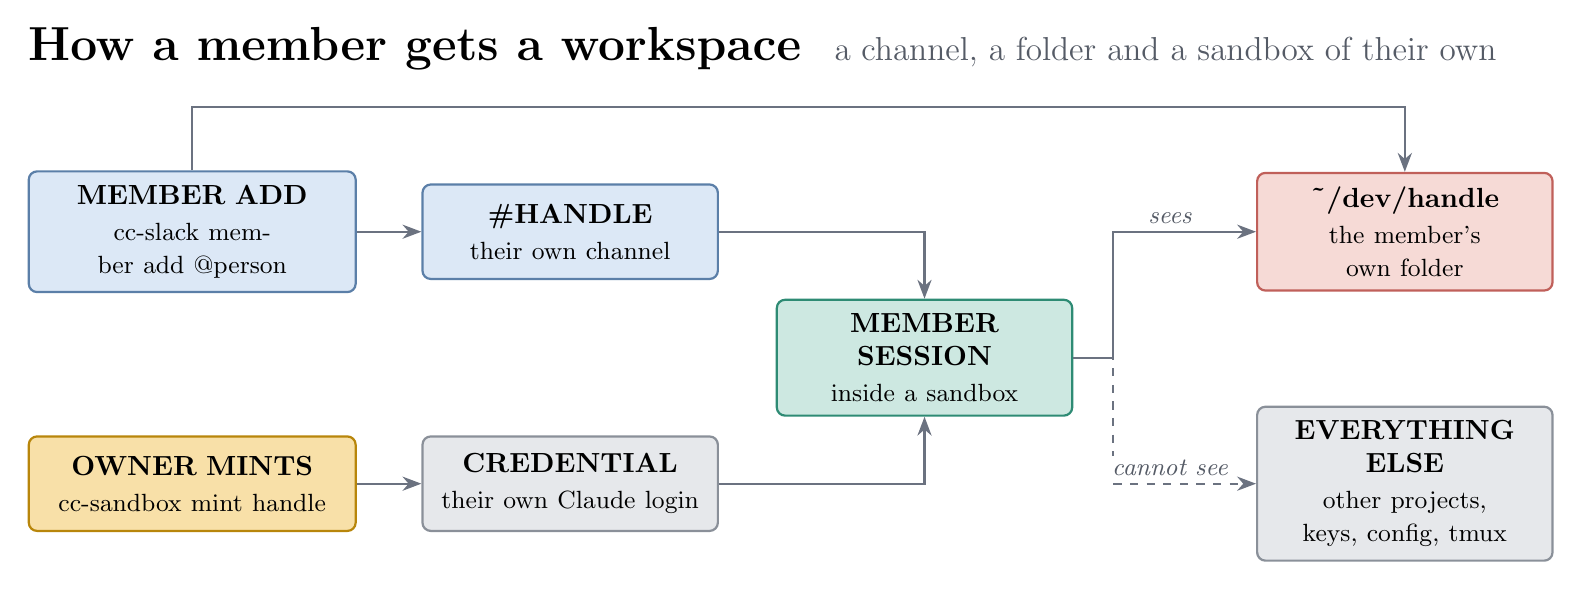
\begin{tikzpicture}
\node[slack, text width=3.8cm] (add) at (0,1.6) {\nd{MEMBER ADD}{cc-slack member add @person}};
\node[person, text width=3.8cm] (mint) at (0,-1.6) {\nd{OWNER MINTS}{cc-sandbox mint handle}};
\node[slack] (ch) at (4.8,1.6) {\nd{\#HANDLE}{their own channel}};
\node[serv] (cred) at (4.8,-1.6) {\nd{CREDENTIAL}{their own Claude login}};
\node[sess] (sess) at (9.3,0) {\nd{MEMBER SESSION}{inside a sandbox}};
\node[code] (dir) at (15.4,1.6) {\nd{\textasciitilde/dev/handle}{the member's own folder}};
\node[serv] (rest) at (15.4,-1.6) {\nd{EVERYTHING ELSE}{other projects, keys, config, tmux}};
\draw[arr] (add) -- (ch);
\draw[arr] (add.north) -- ++(0,0.8) -| (dir.north);
\draw[arr] (mint) -- (cred);
\draw[arr] (ch.east) -| (sess.north);
\draw[arr] (cred.east) -| (sess.south);
\draw[arr] (sess.east) -- ++(0.5,0) |- node[lab, pos=0.7, above=1pt] {sees} (dir.west);
\draw[arr, dashed] (sess.east) -- ++(0.5,0) |- node[lab, pos=0.7, above=1pt] {cannot see} (rest.west);
\titled{How a member gets a workspace}{a channel, a folder and a sandbox of their own}
\end{tikzpicture}
\end{document}
